\chapter{Numerical Application}
\section{Simulation on the Plane}
\subsection{Initial condition}
We consider a Rover on a incline plane. The rover will be put above the plane as the initial position. Then it will fall freely to the plane. The code will simulate the contact and friction between the tyres and the plane. And driving force is put on six wheels. The two front wheel will turn to the right direction.\footnote{Source File Location: siconos/trunk/SandBox/Rover/Rover3DPlane}
\begin{figure}[H]
 \begin{center}
      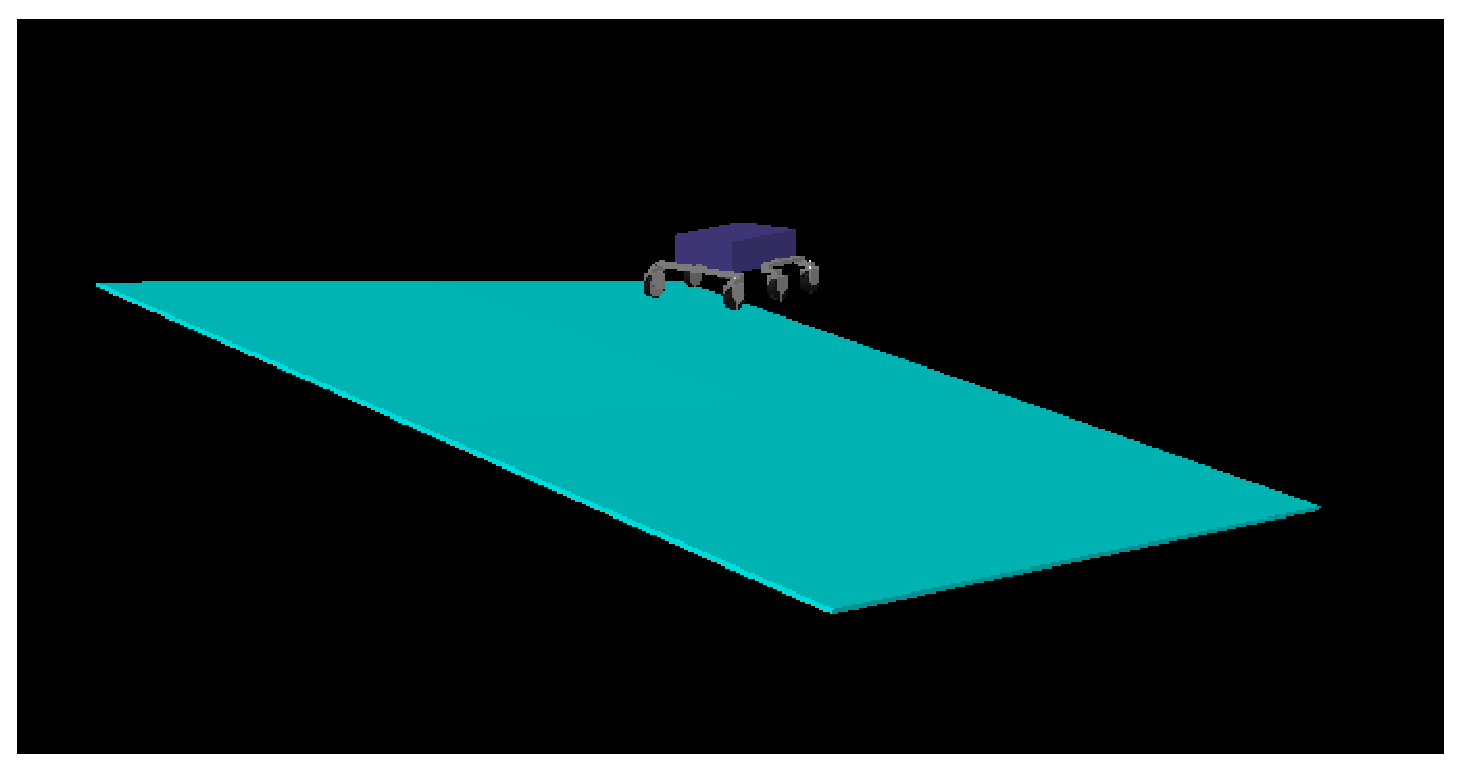
\includegraphics[width=4in]{Chapter5/roverepsplane.eps}
    \caption{Initial condition of RoverPlane model}
  \end{center}
\end{figure}



\subsection{Simulation result}
Beside the VRML animation, we can also export some data to display more details of the movement of the Rover.

\begin{figure}[H]
 \begin{center}
      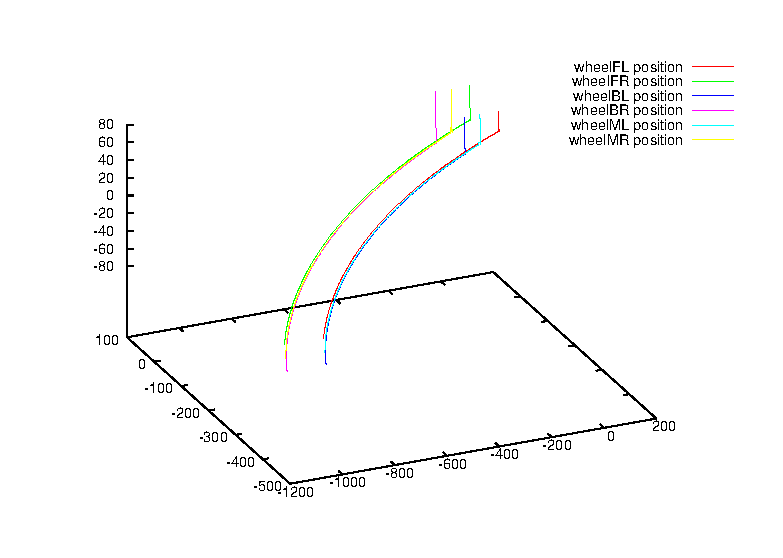
\includegraphics[width=4in]{Chapter5/RoverPlane.eps}
    \caption{Trace of Rover Wheels}
  \end{center}
\end{figure}

\begin{figure}[H]
 \begin{center}
      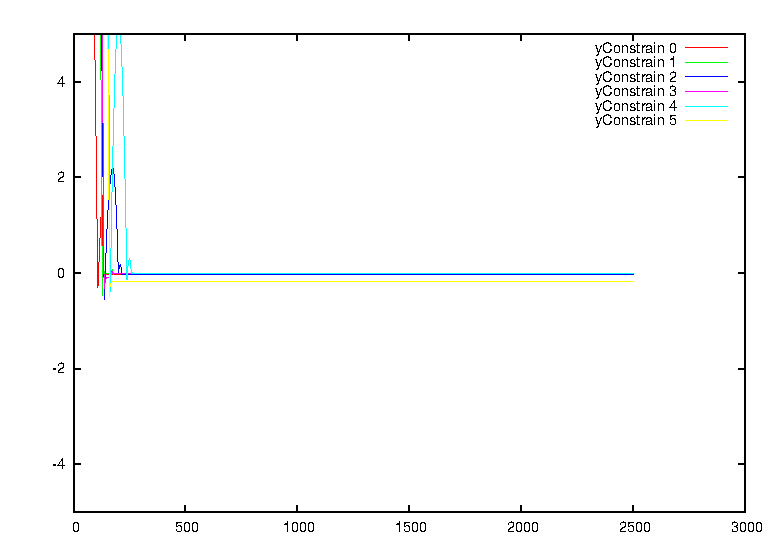
\includegraphics[width=3.5in]{Chapter5/RoverPlaneConstrain.eps}
    \caption{Contact Distance between Wheels and Plane}
    \label{RoverPCons}
  \end{center}
\end{figure}

In the figure \ref{RoverPCons}, we can find that, all the wheels are constrained upon the plane very well.

\begin{figure}[H]
 \begin{center}
      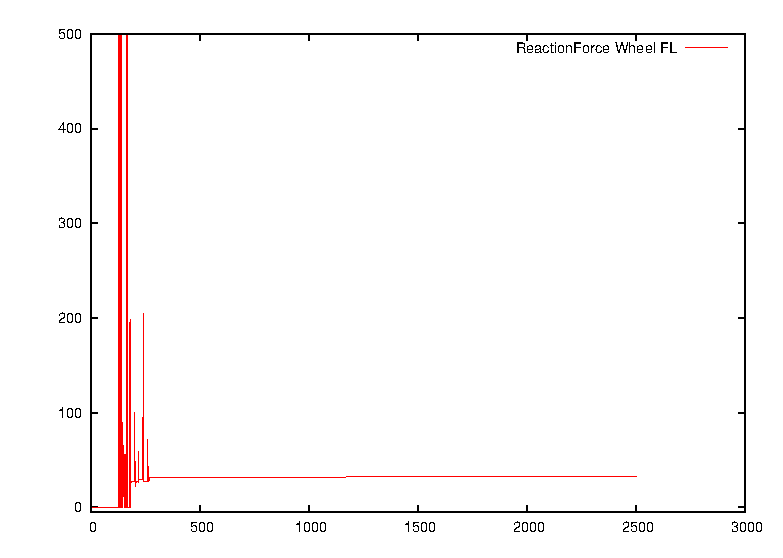
\includegraphics[width=3in]{Chapter5/RoverPlaneReaction.eps}
    \caption{Reaction force of Front Left Wheel}
  \end{center}
\end{figure}

\begin{figure}[H]
 \begin{center}
      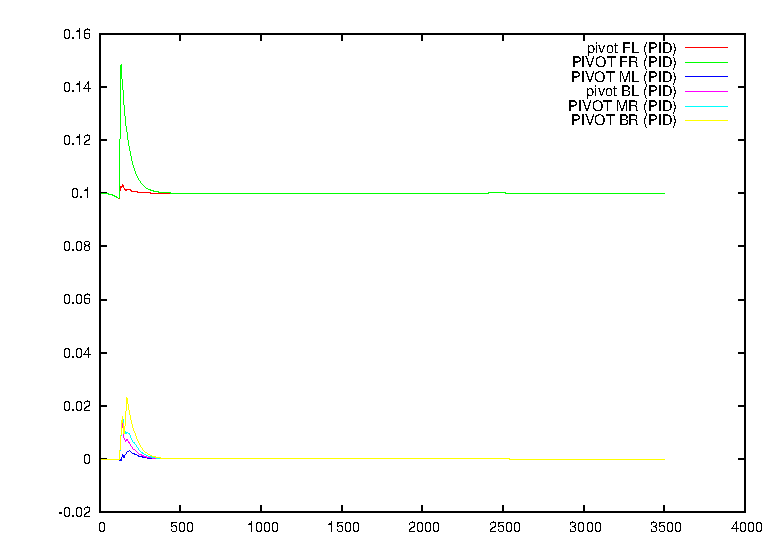
\includegraphics[width=3in]{Chapter5/RoverPlanePID.eps}
    \caption{PID controller}
    \label{PIDfig}
  \end{center}
\end{figure}

Fig \eqref{PIDfig} record the angle of steering system along with time. From the curve,we can find that, the PID controller constrain the steering angle very well.

\section{Simulation on Fixed Spheres}
To simulate Mars Rover on the granular soil, we could use spheres to simulate the granular soil. The figure below shows the simulation of Rover with fixed spheres, to test the validity of our dynamical model.\footnote{Source Files Location: siconos/trunk/SandBox/Rover/Rover3D\_Multi\_Sphere}


\begin{figure}[H]
 \begin{center}
      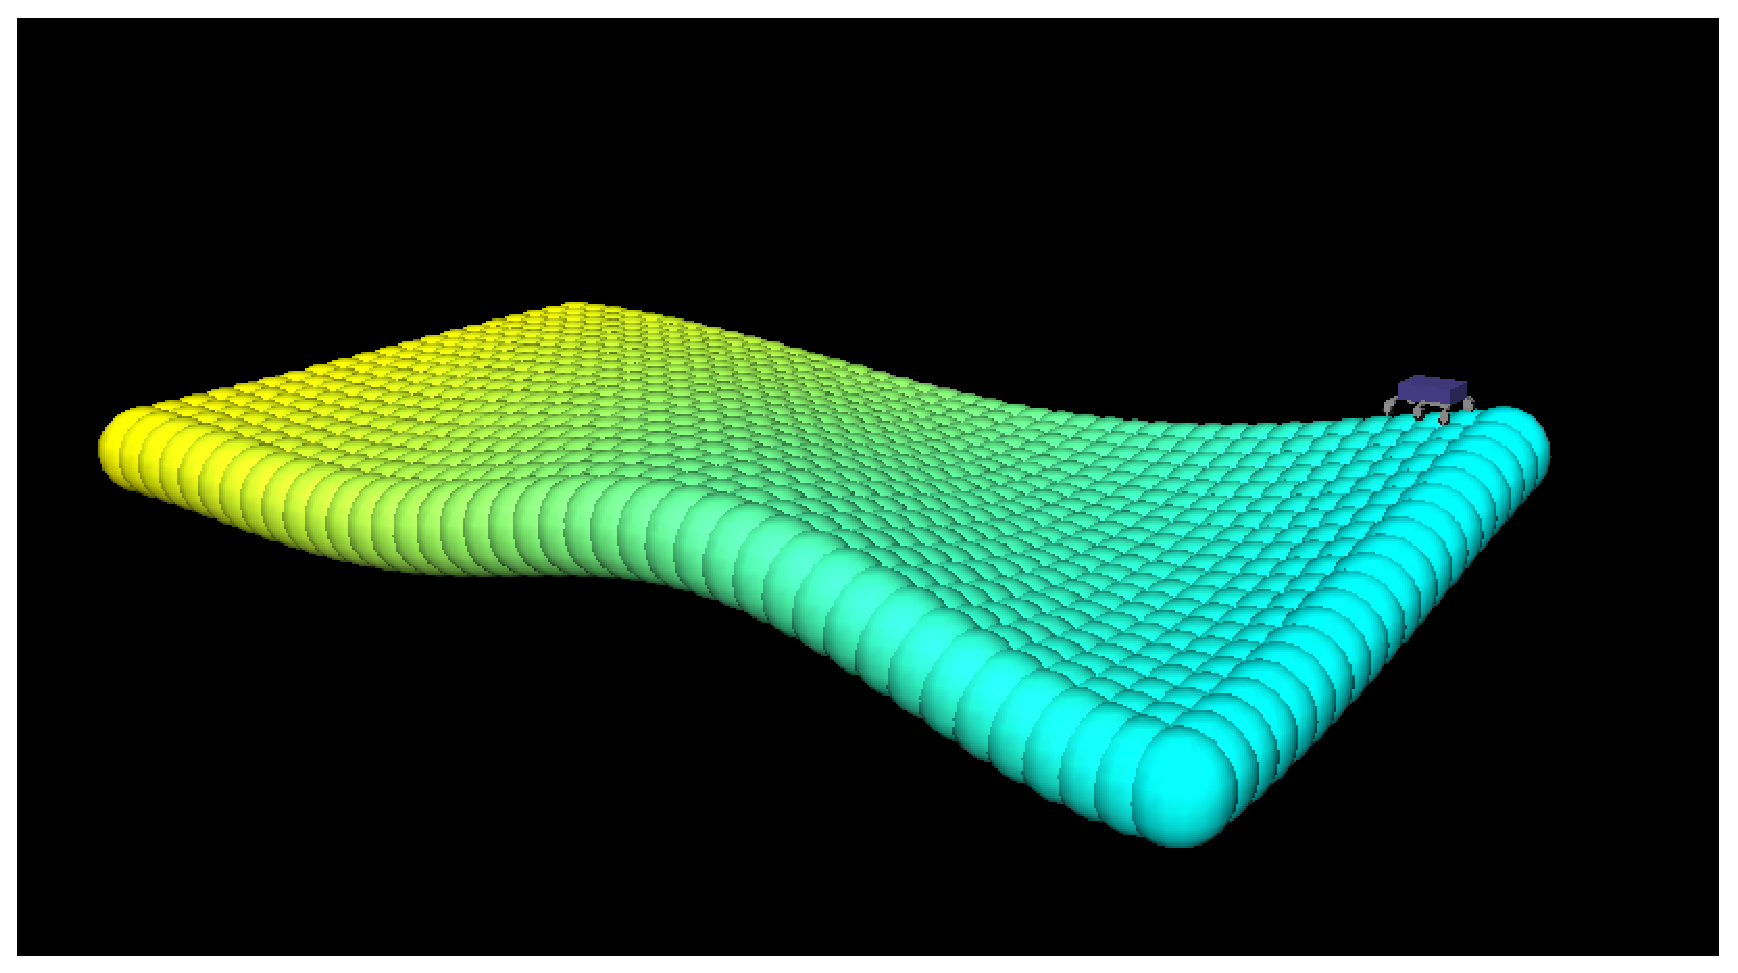
\includegraphics[width=5in]{Chapter5/RoverSpheres.eps}
    \caption{Simulation of Rover with fixed Sphere}
  \end{center}
\end{figure}



